% PARTE 2: EJEMPLOS RESUELTOS Y EJERCICIOS INVERSOS

\section{Ejemplos Resueltos}

\begin{nota}
En esta sección vamos a resolver paso a paso varios problemas con funciones trigonométricas inversas. ¡Presta mucha atención a los detalles y recuerda siempre verificar los rangos!
\end{nota}

% EJEMPLO 1: Calcular arcsen(1/2)
\begin{ejemplo}
\textbf{Ejemplo 1:} Calcular el valor exacto de $\arcsen\left(\frac{1}{2}\right)$.

\textbf{Solución:}

\textbf{Paso 1:} Planteamos la ecuación. Si $y = \arcsen\left(\frac{1}{2}\right)$, entonces necesitamos encontrar el ángulo $y$ tal que:
$$\sen(y) = \frac{1}{2}$$

\textbf{Paso 2:} Recordamos los valores especiales del seno. De nuestro círculo unitario sabemos que:
$$\sen\left(\frac{\pi}{6}\right) = \sen(30°) = \frac{1}{2}$$

\textbf{Paso 3:} Verificamos que esté en el rango correcto del arcoseno. El rango del arcoseno es $\left[-\frac{\pi}{2}, \frac{\pi}{2}\right]$ o $[-90°, 90°]$.

Como $\frac{\pi}{6} = 30°$ está dentro de este rango, ¡es nuestra respuesta!

\textbf{Respuesta final:} $\arcsen\left(\frac{1}{2}\right) = \frac{\pi}{6}$ radianes o $30°$

\textbf{Verificación:}
Comprobemos: $\sen\left(\frac{\pi}{6}\right) = \frac{1}{2}$ ✓

¡Perfecto! Nuestra respuesta es correcta.
\end{ejemplo}

% EJEMPLO 2: Calcular arccos(-√3/2)
\begin{ejemplo}
\textbf{Ejemplo 2:} Determinar $\arccos\left(-\frac{\sqrt{3}}{2}\right)$.

\textbf{Solución:}

\textbf{Paso 1:} Buscamos el ángulo $\theta$ tal que:
$$\cos(\theta) = -\frac{\sqrt{3}}{2}$$

\textbf{Paso 2:} Recordamos que el coseno es negativo en el segundo y tercer cuadrante. Pero ¡ojo! El rango del arcocoseno es $[0, \pi]$ o $[0°, 180°]$, lo que significa que solo consideramos el primer y segundo cuadrante.

\textbf{Paso 3:} Sabemos que $\cos(30°) = \frac{\sqrt{3}}{2}$. Como necesitamos el coseno negativo y debe estar en el segundo cuadrante:
$$\theta = 180° - 30° = 150°$$
O en radianes:
$$\theta = \pi - \frac{\pi}{6} = \frac{5\pi}{6}$$

\textbf{Paso 4:} Verificamos que esté en el rango correcto: $\frac{5\pi}{6}$ está en $[0, \pi]$ ✓

\textbf{Respuesta:} $\arccos\left(-\frac{\sqrt{3}}{2}\right) = \frac{5\pi}{6}$ radianes o $150°$

\begin{center}
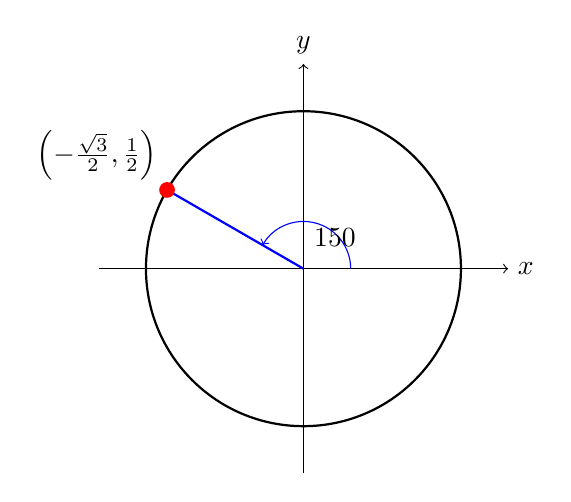
\begin{tikzpicture}[scale=2]
    % Círculo unitario
    \draw[thick] (0,0) circle (1);
    % Ejes
    \draw[->] (-1.3,0) -- (1.3,0) node[right] {$x$};
    \draw[->] (0,-1.3) -- (0,1.3) node[above] {$y$};
    % Ángulo
    \draw[thick, blue] (0,0) -- (-0.866,0.5);
    \draw[blue, ->] (0.3,0) arc (0:150:0.3);
    \node at (0.2,0.2) {$150°$};
    % Punto
    \fill[red] (-0.866,0.5) circle (0.05);
    \node[above left] at (-0.866,0.5) {$\left(-\frac{\sqrt{3}}{2}, \frac{1}{2}\right)$};
\end{tikzpicture}
\end{center}
\end{ejemplo}

% EJEMPLO 3: Calcular sen(arctan(3/4))
\begin{ejemplo}
\textbf{Ejemplo 3:} Calcular $\sen(\arctan(3/4))$ sin usar calculadora.

\textbf{Solución:}

\textbf{Paso 1:} Sea $\theta = \arctan(3/4)$. Esto significa que $\tan(\theta) = \frac{3}{4}$.

\textbf{Paso 2:} Recordamos que $\tan(\theta) = \frac{\text{opuesto}}{\text{adyacente}}$. Entonces podemos dibujar un triángulo rectángulo donde:
\begin{itemize}
\item Cateto opuesto = 3
\item Cateto adyacente = 4
\end{itemize}

\begin{center}
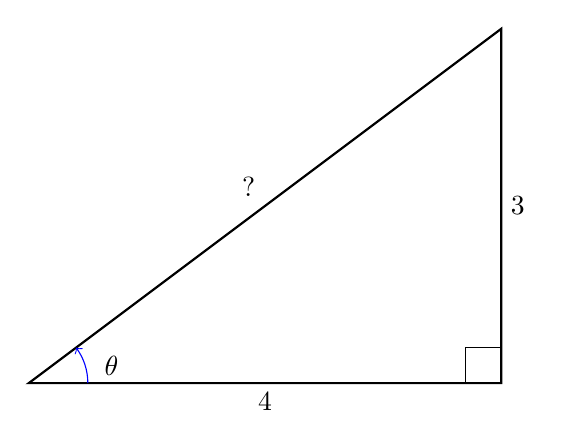
\begin{tikzpicture}[scale=1.5]
    % Triángulo
    \draw[thick] (0,0) -- (4,0) -- (4,3) -- cycle;
    % Ángulo recto
    \draw (3.7,0) -- (3.7,0.3) -- (4,0.3);
    % Ángulo theta
    \draw[blue, ->] (0.5,0) arc (0:37:0.5);
    \node at (0.7,0.15) {$\theta$};
    % Etiquetas
    \node[below] at (2,0) {4};
    \node[right] at (4,1.5) {3};
    \node[above left] at (2,1.5) {?};
\end{tikzpicture}
\end{center}

\textbf{Paso 3:} Usamos el teorema de Pitágoras para encontrar la hipotenusa:
$$\text{hipotenusa} = \sqrt{3^2 + 4^2} = \sqrt{9 + 16} = \sqrt{25} = 5$$

\textbf{Paso 4:} Ahora calculamos $\sen(\theta)$:
$$\sen(\theta) = \frac{\text{opuesto}}{\text{hipotenusa}} = \frac{3}{5}$$

\textbf{Respuesta:} $\sen(\arctan(3/4)) = \frac{3}{5}$

¡Fíjate que no necesitamos saber el valor exacto del ángulo para resolver este problema!
\end{ejemplo}

% EJEMPLO 4: Simplificar cos(arcsen(x))
\begin{ejemplo}
\textbf{Ejemplo 4:} Simplificar $\cos(\arcsen(x))$ donde $-1 \leq x \leq 1$.

\textbf{Solución:}

\textbf{Paso 1:} Sea $\theta = \arcsen(x)$, entonces $\sen(\theta) = x$ y $-\frac{\pi}{2} \leq \theta \leq \frac{\pi}{2}$.

\textbf{Paso 2:} Usamos la identidad pitagórica fundamental:
$$\sen^2(\theta) + \cos^2(\theta) = 1$$

\textbf{Paso 3:} Sustituimos $\sen(\theta) = x$:
$$x^2 + \cos^2(\theta) = 1$$

\textbf{Paso 4:} Despejamos $\cos(\theta)$:
$$\cos^2(\theta) = 1 - x^2$$
$$\cos(\theta) = \pm\sqrt{1 - x^2}$$

\textbf{Paso 5:} ¿Signo positivo o negativo? Como $\theta$ está en el rango $\left[-\frac{\pi}{2}, \frac{\pi}{2}\right]$, estamos en el cuarto o primer cuadrante, donde el coseno es SIEMPRE positivo. Por lo tanto:

$$\cos(\theta) = \sqrt{1 - x^2}$$

\textbf{Respuesta:} $\cos(\arcsen(x)) = \sqrt{1 - x^2}$ para $-1 \leq x \leq 1$

\textbf{Ejemplo numérico:} Si $x = \frac{3}{5}$, entonces:
$$\cos\left(\arcsen\left(\frac{3}{5}\right)\right) = \sqrt{1 - \left(\frac{3}{5}\right)^2} = \sqrt{1 - \frac{9}{25}} = \sqrt{\frac{16}{25}} = \frac{4}{5}$$
\end{ejemplo}

% EJEMPLO 5: Resolver ecuación con funciones inversas
\begin{ejemplo}
\textbf{Ejemplo 5:} Resolver la ecuación $\arctan(x) + \arctan(2x) = \frac{\pi}{4}$.

\textbf{Solución:}

\textbf{Paso 1:} Usaremos la fórmula de suma para la arcotangente:
$$\arctan(a) + \arctan(b) = \arctan\left(\frac{a + b}{1 - ab}\right)$$
siempre que $ab < 1$.

\textbf{Paso 2:} Aplicamos la fórmula con $a = x$ y $b = 2x$:
$$\arctan(x) + \arctan(2x) = \arctan\left(\frac{x + 2x}{1 - x \cdot 2x}\right) = \arctan\left(\frac{3x}{1 - 2x^2}\right)$$

\textbf{Paso 3:} Como esto debe ser igual a $\frac{\pi}{4}$, y sabemos que $\tan\left(\frac{\pi}{4}\right) = 1$:
$$\arctan\left(\frac{3x}{1 - 2x^2}\right) = \arctan(1)$$

\textbf{Paso 4:} Por lo tanto:
$$\frac{3x}{1 - 2x^2} = 1$$

\textbf{Paso 5:} Resolvemos la ecuación:
$$3x = 1 - 2x^2$$
$$2x^2 + 3x - 1 = 0$$

\textbf{Paso 6:} Usamos la fórmula cuadrática:
$$x = \frac{-3 \pm \sqrt{9 + 8}}{4} = \frac{-3 \pm \sqrt{17}}{4}$$

\textbf{Paso 7:} Obtenemos dos soluciones:
$$x_1 = \frac{-3 + \sqrt{17}}{4} \approx 0.281$$
$$x_2 = \frac{-3 - \sqrt{17}}{4} \approx -1.781$$

\textbf{Paso 8:} Verificamos que $2x^2 < 1$ para que la fórmula sea válida:
- Para $x_1 \approx 0.281$: $2(0.281)^2 \approx 0.158 < 1$ ✓
- Para $x_2 \approx -1.781$: $2(-1.781)^2 \approx 6.34 > 1$ ✗

\textbf{Respuesta:} $x = \frac{-3 + \sqrt{17}}{4}$

\textbf{Verificación:} Puedes comprobar con calculadora que:
$$\arctan(0.281) + \arctan(0.562) \approx 0.274 + 0.512 = 0.786 \approx \frac{\pi}{4}$$ ✓
\end{ejemplo}

\section{Ejercicios Inversos (Pensamiento Creativo)}

\begin{nota}
En estos ejercicios, en lugar de resolver un problema dado, debes \textbf{crear} o \textbf{diseñar} algo que cumpla ciertas condiciones. Esto desarrolla tu creatividad matemática y comprensión profunda del tema. ¡Es como ser el profesor en lugar del estudiante!
\end{nota}

% EJERCICIO INVERSO 1
\begin{ejercicio}
\textbf{Ejercicio Inverso 1: El Arquitecto de Identidades}

Diseña una expresión que involucre dos funciones trigonométricas inversas diferentes cuyo valor sea exactamente $\frac{\pi}{2}$.

Por ejemplo, podrías usar $\arcsen(?) + \arccos(?) = \frac{\pi}{2}$.

\textbf{Requisitos:}
\begin{itemize}
\item Debe usar al menos dos funciones inversas diferentes
\item El resultado debe ser exacto (no aproximado)
\item Justifica por qué tu expresión funciona
\item Bonus: ¿Puedes crear una que use tres funciones inversas?
\end{itemize}
\end{ejercicio}

% EJERCICIO INVERSO 2
\begin{ejercicio}
\textbf{Ejercicio Inverso 2: El Ingeniero de Drones}

Crea un problema aplicado de la vida real donde sea necesario usar arcotangente para encontrar un ángulo.

\textbf{Contexto sugerido:} Un dron debe volar desde el punto A hasta el punto B evitando obstáculos. Necesitas calcular el ángulo de navegación.

\textbf{Requisitos:}
\begin{itemize}
\item Contexto realista (navegación, arquitectura, física, videojuegos, etc.)
\item Datos numéricos específicos
\item Incluye un diagrama de la situación
\item La solución debe usar arctan o arctan2
\item Explica por qué es mejor usar funciones inversas que medir directamente
\end{itemize}
\end{ejercicio}

% EJERCICIO INVERSO 3
\begin{ejercicio}
\textbf{Ejercicio Inverso 3: El Explorador de Patrones}

Encuentra un valor de $x$ tal que $\arcsen(x) + \arccos(x)$ tenga un valor interesante o especial.

\textbf{Requisitos:}
\begin{itemize}
\item Explica por qué elegiste ese valor de $x$
\item Calcula el resultado exacto
\item Generaliza: ¿funciona para cualquier $x$ en el dominio?
\item ¿Qué pasa si cambias la suma por una resta?
\end{itemize}
\end{ejercicio}

% EJERCICIO INVERSO 4
\begin{ejercicio}
\textbf{Ejercicio Inverso 4: El Detective Matemático}

Inventa una ecuación que involucre $\arctan(x)$ y que tenga exactamente dos soluciones: una positiva y una negativa con el mismo valor absoluto.

\textbf{Requisitos:}
\begin{itemize}
\item La ecuación debe ser diferente a los ejemplos vistos
\item Debe tener soluciones simétricas (tipo $x = \pm a$)
\item Proporciona el proceso de resolución completo
\item Explica geométricamente por qué hay simetría
\end{itemize}
\end{ejercicio}

% EJERCICIO INVERSO 5
\begin{ejercicio}
\textbf{Ejercicio Inverso 5: El Diseñador de Funciones}

Crea una función compuesta $f(x) = \arcsen(g(x))$ donde $g(x)$ sea una función racional (cociente de polinomios) tal que el dominio de $f$ sea exactamente el intervalo $[-2, 2]$.

\textbf{Requisitos:}
\begin{itemize}
\item Define explícitamente $g(x)$
\item Demuestra que el dominio de $f$ es $[-2, 2]$
\item Grafica tu función (puedes hacerlo a mano o describir su forma)
\item ¿Cuál es el rango de tu función?
\end{itemize}
\end{ejercicio}

\section{Soluciones de los Ejercicios Inversos}

\begin{solucion}
\textbf{Solución Ejercicio Inverso 1: El Arquitecto de Identidades}

Hay varias respuestas creativas posibles. Aquí te muestro tres:

\textbf{Opción 1:} La más elegante
$$\arcsen(x) + \arccos(x) = \frac{\pi}{2} \quad \text{para cualquier } x \in [-1, 1]$$

\textbf{Justificación:} Si $\theta = \arcsen(x)$, entonces $\sen(\theta) = x$ y $\theta \in \left[-\frac{\pi}{2}, \frac{\pi}{2}\right]$.
El ángulo complementario $\frac{\pi}{2} - \theta$ tiene la propiedad de que:
$$\cos\left(\frac{\pi}{2} - \theta\right) = \sen(\theta) = x$$
Por lo tanto, $\arccos(x) = \frac{\pi}{2} - \theta = \frac{\pi}{2} - \arcsen(x)$.

\textbf{Opción 2:} Usando valores específicos
$$\arcsen\left(\frac{\sqrt{2}}{2}\right) + \arctan(1) = \frac{\pi}{4} + \frac{\pi}{4} = \frac{\pi}{2}$$

\textbf{Opción 3:} Con tres funciones (bonus)
$$\arcsen\left(\frac{1}{2}\right) + \arccos\left(\frac{\sqrt{3}}{2}\right) + \arctan(0) = \frac{\pi}{6} + \frac{\pi}{6} + 0 = \frac{\pi}{2}$$
\end{solucion}

\begin{solucion}
\textbf{Solución Ejercicio Inverso 2: El Ingeniero de Drones}

\textbf{Problema creado:}
Un dron de entrega está en la azotea de un edificio de 50 metros de altura en la posición $(0, 0, 50)$. Debe entregar un paquete en otro edificio de 30 metros de altura ubicado en la posición $(80, 60, 30)$ metros. El dron debe calcular su ángulo de navegación horizontal y el ángulo de descenso.

\begin{center}
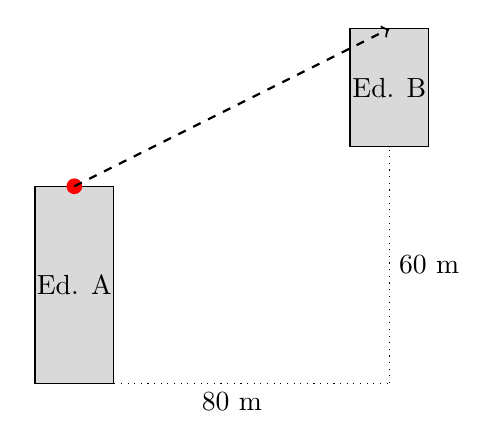
\begin{tikzpicture}[scale=0.05]
    % Edificio 1
    \draw[fill=gray!30] (0,0) rectangle (20,50);
    \node at (10,25) {Ed. A};
    % Edificio 2
    \draw[fill=gray!30] (80,60) rectangle (100,90);
    \node at (90,75) {Ed. B};
    % Dron
    \fill[red] (10,50) circle (2);
    % Trayectoria
    \draw[dashed, thick, ->] (10,50) -- (90,90);
    % Proyección en el plano
    \draw[dotted] (10,0) -- (90,0);
    \draw[dotted] (90,0) -- (90,60);
    % Etiquetas
    \node[below] at (50,0) {80 m};
    \node[right] at (90,30) {60 m};
\end{tikzpicture}
\end{center}

\textbf{Solución:}

1) \textbf{Ángulo de navegación horizontal:}
$$\theta_h = \arctan\left(\frac{60}{80}\right) = \arctan\left(\frac{3}{4}\right) \approx 36.87°$$

2) \textbf{Distancia horizontal:}
$$d_h = \sqrt{80^2 + 60^2} = \sqrt{6400 + 3600} = 100 \text{ metros}$$

3) \textbf{Ángulo de descenso:}
$$\theta_v = \arctan\left(\frac{50 - 30}{100}\right) = \arctan\left(\frac{1}{5}\right) \approx 11.31°$$

\textbf{Por qué usar funciones inversas:} Es imposible medir estos ángulos directamente desde el dron. El GPS proporciona coordenadas, y las funciones inversas permiten calcular los ángulos de navegación necesarios.
\end{solucion}

\begin{solucion}
\textbf{Solución Ejercicio Inverso 3: El Explorador de Patrones}

\textbf{Descubrimiento sorprendente:} Para CUALQUIER valor de $x$ en $[-1, 1]$:
$$\arcsen(x) + \arccos(x) = \frac{\pi}{2}$$

\textbf{Demostración:}
Sea $\alpha = \arcsen(x)$, entonces $\sen(\alpha) = x$ y $-\frac{\pi}{2} \leq \alpha \leq \frac{\pi}{2}$.

Por identidad de ángulos complementarios:
$$\cos\left(\frac{\pi}{2} - \alpha\right) = \sen(\alpha) = x$$

Como $\frac{\pi}{2} - \alpha \in [0, \pi]$ (el rango del arccos), tenemos:
$$\arccos(x) = \frac{\pi}{2} - \alpha = \frac{\pi}{2} - \arcsen(x)$$

Por lo tanto: $\arcsen(x) + \arccos(x) = \frac{\pi}{2}$ ¡siempre!

\textbf{¿Qué pasa con la resta?}
$$\arcsen(x) - \arccos(x) = 2\arcsen(x) - \frac{\pi}{2}$$

Por ejemplo:
- Si $x = 0$: $\arcsen(0) - \arccos(0) = 0 - \frac{\pi}{2} = -\frac{\pi}{2}$
- Si $x = 1$: $\arcsen(1) - \arccos(1) = \frac{\pi}{2} - 0 = \frac{\pi}{2}$
- Si $x = -1$: $\arcsen(-1) - \arccos(-1) = -\frac{\pi}{2} - \pi = -\frac{3\pi}{2}$
\end{solucion}

\begin{solucion}
\textbf{Solución Ejercicio Inverso 4: El Detective Matemático}

\textbf{Ecuación creada:}
$$\arctan(x^2 - 1) = \arctan(2x)$$

\textbf{Resolución:}
Como las funciones arctan son iguales, sus argumentos deben ser iguales:
$$x^2 - 1 = 2x$$
$$x^2 - 2x - 1 = 0$$

Usando la fórmula cuadrática:
$$x = \frac{2 \pm \sqrt{4 + 4}}{2} = \frac{2 \pm 2\sqrt{2}}{2} = 1 \pm \sqrt{2}$$

\textbf{Soluciones:}
- $x_1 = 1 + \sqrt{2} \approx 2.414$ (positiva)
- $x_2 = 1 - \sqrt{2} \approx -0.414$ (negativa)

¡Ups! Estas no son simétricas. Intentemos otra ecuación:

\textbf{Mejor ecuación:}
$$\arctan(x) + \arctan(x^3) = \arctan(2)$$

Después de manipulación algebraica (usando la fórmula de suma), obtenemos:
$$x^4 - 2x^2 + 1 = 0$$
$$(x^2 - 1)^2 = 0$$
$$x^2 = 1$$
$$x = \pm 1$$

¡Perfecto! Soluciones simétricas.

\textbf{Explicación geométrica:} La simetría ocurre porque la función $f(x) = \arctan(x) + \arctan(x^3)$ es impar: $f(-x) = -f(x)$. Si $a$ es solución de $f(x) = c$, entonces $-a$ es solución de $f(x) = -c$.
\end{solucion}

\begin{solucion}
\textbf{Solución Ejercicio Inverso 5: El Diseñador de Funciones}

\textbf{Función creada:}
$$f(x) = \arcsen\left(\frac{x}{2}\right)$$

donde $g(x) = \frac{x}{2}$

\textbf{Demostración del dominio:}
Para que $\arcsen(g(x))$ esté definida, necesitamos:
$$-1 \leq g(x) \leq 1$$
$$-1 \leq \frac{x}{2} \leq 1$$
$$-2 \leq x \leq 2$$

Por lo tanto, el dominio de $f$ es exactamente $[-2, 2]$. ✓

\textbf{Rango de la función:}
Como $x \in [-2, 2]$, entonces $\frac{x}{2} \in [-1, 1]$.
El rango del arcoseno es $\left[-\frac{\pi}{2}, \frac{\pi}{2}\right]$.
Por lo tanto, el rango de $f$ es $\left[-\frac{\pi}{2}, \frac{\pi}{2}\right]$.

\textbf{Gráfica:}

\begin{center}
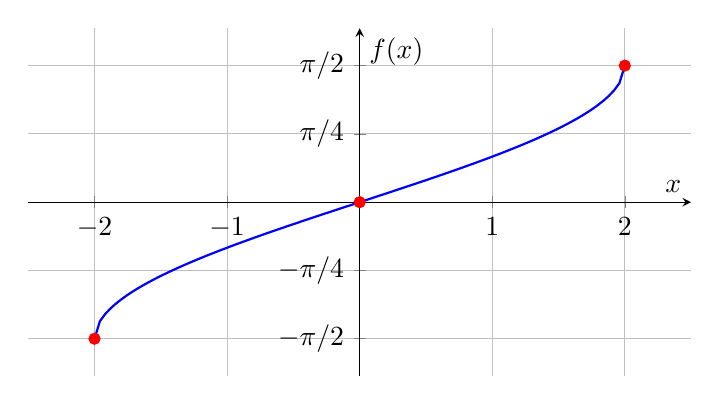
\begin{tikzpicture}
\begin{axis}[
    xlabel={$x$},
    ylabel={$f(x)$},
    xmin=-2.5, xmax=2.5,
    ymin=-2, ymax=2,
    axis lines=middle,
    grid=major,
    width=10cm,
    height=6cm,
    xtick={-2,-1,0,1,2},
    ytick={-1.57, -0.785, 0, 0.785, 1.57},
    yticklabels={$-\pi/2$, $-\pi/4$, $0$, $\pi/4$, $\pi/2$},
]
\addplot[domain=-2:2, samples=100, thick, blue] {asin(x/2)*pi/180};
\addplot[only marks, red] coordinates {(-2,-1.57) (0,0) (2,1.57)};
\end{axis}
\end{tikzpicture}
\end{center}

La función es creciente, pasa por el origen, y tiene forma de S estirada.

\textbf{Función alternativa más interesante:}
$$f(x) = \arcsen\left(\frac{x^2 - 4}{5}\right)$$

Esta también tiene dominio $[-2, 2]$ pero no es monótona, creando una curva más interesante.
\end{solucion}